\documentclass{article}
\usepackage{tikz}
\usetikzlibrary{patterns,fadings}
\usetikzlibrary{calc}
\usepackage{color}
\begin{document}
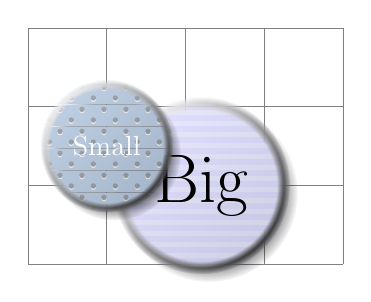
\begin{tikzpicture}
[
% Define an interesting style
button/.style={
% First preaction: Fuzzy shadow
preaction={fill=black,path fading=circle with fuzzy edge 20 percent,
opacity=.5,transform canvas={xshift=1mm,yshift=-1mm}},
% Second preaction: Background pattern
preaction={pattern=#1,
path fading=circle with fuzzy edge 15 percent},
% Third preaction: Make background shiny
preaction={top color=white,
bottom color=black!50,
shading angle=45,
path fading=circle with fuzzy edge 15 percent,
opacity=0.2},
% Fourth preaction: Make edge especially shiny
preaction={path fading=fuzzy ring 15 percent,
top color=black!5,
bottom color=black!80,
shading angle=45},
inner sep=2ex
},
button/.default=horizontal lines light blue,
circle
]
\draw [help lines] (0,0) grid (4,3);
\node [button] at (2.2,1) {\Huge Big};
\node [button=crosshatch dots light steel blue,
text=white] at (1,1.5) {Small};
\end{tikzpicture}



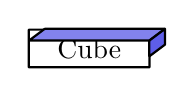
\begin{tikzpicture}
    % Settings
    \definecolor{CUBE}{rgb}{0.3,0.3,0.9};
    \coordinate (CenterPoint) at (0,0);
    \def\width{1.5cm};
    \def\height{0.2cm};
    \def\textborder{0.1cm};
    \def\xslant{0.2cm};
    \def\yslant{0.15cm};
    \def\rounding{0.2pt};
    % Drawing
    \node[thick, draw,
          minimum height  = \height,
          minimum width   = \width,
          text width      = {\width-2*\textborder},
          align           = center,
        %   fill            = CUBE!50,
          rounded corners = \rounding]
          at (CenterPoint) {Cube}; % TEXT HERE?
    % "3D" top
    \draw [rounded corners = \rounding, thick, fill=CUBE!70] %
        ($(CenterPoint) + (-\width/2. - 2*\rounding, \height/2.)$) -- %
        ($(CenterPoint) + (-\width/2. + \xslant - 2*\rounding, \height/2. + \yslant)$) -- %
        ($(CenterPoint) + (\width/2. + \xslant + 2*\rounding, \height/2. + \yslant)$) -- %
        ($(CenterPoint) + (\width/2. + 2*\rounding, \height/2.)$) -- %
        cycle;
    % "3D" side
    \draw [rounded corners = \rounding, thick, fill=CUBE!90] %
        ($(CenterPoint) + (\width/2. + \xslant + 2*\rounding, \height/2. + \yslant)$) -- %
        ($(CenterPoint) + (\width/2. + 2*\rounding, \height/2.)$) -- %
        ($(CenterPoint) + (\width/2. + 2*\rounding, -\height/2.)$) -- %
        ($(CenterPoint) + (\width/2. + \xslant + 2*\rounding, -\height/2. + \yslant)$) -- %
        cycle;
    \end{tikzpicture}

\end{document}